\documentclass[conference]{IEEEtran}
\IEEEoverridecommandlockouts
% The preceding line is only needed to identify funding in the first footnote. If that is unneeded, please comment it out.
\usepackage{cite}
\usepackage{amsmath,amssymb,amsfonts}
\usepackage{algorithmic}
\usepackage{graphicx}
\usepackage{textcomp}
\usepackage{xcolor}
\def\BibTeX{{\rm B\kern-.05em{\sc i\kern-.025em b}\kern-.08em
    T\kern-.1667em\lower.7ex\hbox{E}\kern-.125emX}}
\begin{document}

\title{Phishing Protection for Companies: A Comprehensive Analysis of Training Methods and Campaign Strategies\\
{\footnotesize \textsuperscript{}}
\thanks{Identify applicable funding agency here. If none, delete this.}
}

\author{
\IEEEauthorblockN{1\textsuperscript{st} Yerassylbek Makhsatbekov}
\IEEEauthorblockA{
Astana City, Kazakhstan \\
212538@astanait.edu.kz}
\and
\IEEEauthorblockN{2\textsuperscript{nd} Beybars Kazbekov}
\IEEEauthorblockA{
Astana City, Kazakhstan \\
212227@astanait.edu.kz}
\and
\IEEEauthorblockN{3\textsuperscript{rd} Aknar Asanov}
\IEEEauthorblockA{
Astana City, Kazakhstan \\
212139@astanait.edu.kz}
\and
}

\maketitle

\begin{abstract}Because of the advancements in web, mobile, and social network technology, phishing is becoming a more significant issue in the online world. The main focus of earlier phishing taxonomies was on basic phishing mechanisms; new attack techniques, target settings, and defenses for novel forms of phishing were disregarded. This survey looks at phishing attempts and counter-attack strategies created for both new and established platforms, including social media and mobile websites, in addition to more conventional ones like email and webpages. We provide analysis that covers attack techniques, defenses, target environment, and communications, taking a comprehensive approach to phishing. In addition to offering suggestions for creating efficient techniques for identifying and thwarting phishing in various contexts, the analysis will facilitate practitioners' assessment and choice of tools, features, and methods for tackling particular phishing issues.
\end{abstract}

\begin{IEEEkeywords}
phishing mitigation technique, social engineering, security chain, cyber attack, security, target vulnerability,email classification, phishing attack detection
\end{IEEEkeywords}

\section{Introduction}
Phishing attacks, characterized by deceptive attempts to acquire sensitive information, have evolved into highly sophisticated threats. According to Anderson (2020), these attacks have seen a significant increase in sophistication, posing a substantial danger to organizations worldwide. Cybercriminals continually refine their tactics, making it imperative for companies to fortify their defenses against these evolving threats. These attacks are increasingly sophisticated, making it imperative for companies to fortify their defenses.

The primary objective of this research paper is to provide a comprehensive examination of the training methods and campaign strategies available to organizations for safeguarding their sensitive information against phishing attacks. By assessing the effectiveness of these approaches, we aim to equip companies with the knowledge and tools necessary to mitigate the risks associated with phishing. The primary objective of this research paper is to provide a comprehensive examination of training methods and campaign strategies aimed at mitigating the risks posed by increasingly sophisticated phishing attacks. In a digital landscape where phishing attacks have grown in complexity and frequency (Anderson, 2020), our research aims to equip organizations with the knowledge and tools necessary to effectively combat these evolving threats.

This paper will explore a wide range of training methods and campaign strategies employed by organizations to counter phishing threats. The analysis encompasses various aspects, including their effectiveness, challenges, and best practices. It offers insights into the evolving tactics used by cybercriminals and the impact of phishing attacks on companies, all within the context of corporate environments.

\section{Phishing Threat Landscape}

\subsection{Types of Phishing Attacks}

Phishing attacks encompass a range of deceptive tactics used by cybercriminals to infiltrate organizations. This section delves into the various types of phishing attacks, including but not limited to:

\subsubsection{Spear Phishing}
Spear phishing is a highly targeted attack directed at specific individuals or departments within an organization, often involving extensive research to craft convincing messages (SANS Institute, 2020).

\subsubsection{Business Email Compromise (BEC)}
Business Email Compromise involves the impersonation of high-ranking executives or business partners to trick employees into authorizing financial transactions or revealing sensitive information (FBI, 2022).

\subsubsection{CEO Fraud}
Impersonation of high-ranking executives or business partners to trick employees into authorizing financial transactions or revealing sensitive information.

\subsubsection{Credential Phishing}
Attempts to steal login credentials, such as usernames and passwords, by posing as a trustworthy entity.

\subsubsection{Pharming}
Redirecting users to fraudulent websites that mimic legitimate ones, thereby harvesting sensitive data.

\subsubsection{Vishing (Voice Phishing)}
Deceptive phone calls aimed at extracting sensitive information, often in conjunction with other phishing methods.

\subsubsection{Smishing (SMS Phishing)}
The use of text messages to deceive recipients into taking specific actions, often including links or phone numbers to call.

\subsection{Impact on Companies}
Phishing attacks can have profound repercussions on businesses, including:
\subsubsection{Data Breaches}
Unauthorized access to sensitive data, which can lead to data leaks, compliance violations, and reputational damage.

\subsubsection{Financial Losses}
Scams, such as CEO fraud, can result in significant financial losses if funds are transferred to fraudulent accounts.

\subsubsection{Reputation Damage}
Phishing incidents can tarnish a company's reputation, eroding trust among clients, partners, and employees.

\subsubsection{Operational Disruption}
Successful attacks can disrupt normal business operations, affecting productivity and causing downtime.

\subsubsection{Legal and Regulatory Consequences}
Non-compliance with data protection regulations can lead to legal penalties and regulatory scrutiny.

\subsection{Evolving Tactics}
Phishing tactics are constantly evolving, adapting to technological advancements and user behaviors. This section explores the dynamic nature of phishing, including:

\subsubsection{Social Engineering}
Phishers use psychological manipulation to exploit human vulnerabilities, often leveraging current events, emotions, or trust.

\subsubsection{Advanced Spoofing Techniques}
Attackers employ sophisticated email spoofing, making it challenging to distinguish phishing emails from legitimate ones.

\subsubsection{Malware Distribution}
Phishing emails often serve as vectors for malware delivery, including ransomware, keyloggers, and spyware.

\subsubsection{Zero-Day Exploits}
Some phishing attacks leverage previously unknown vulnerabilities (zero-days) in software or systems, making them harder to detect and mitigate.

\subsubsection{ Multi-Channel Attacks}
Phishing attacks can span multiple communication channels, such as email, text messages, phone calls, and even social media.

Understanding the evolving tactics and their impact is essential for organizations to develop effective countermeasures against phishing threats.

\section{ Training Methods }\label{AA}
Phishing protection within companies relies on an array of training methods to equip employees with the knowledge and skills to recognize and respond to phishing threats effectively. This section delves into the various training methods used in corporate environments:

\subsection{Employee Awareness Training}
Employee awareness training is a fundamental component of any phishing protection strategy. It involves educating employees about the different forms of phishing attacks, the tactics employed by cybercriminals, and the potential risks associated with falling victim to these attacks. This training fosters a sense of responsibility among employees and empowers them to be vigilant and report suspicious activities promptly.

\subsection{Simulated Phishing Exercises}
Simulated phishing exercises provide employees with practical experience in identifying and handling phishing attempts. These exercises involve the creation and deployment of simulated phishing emails, which mimic real-world threats. By monitoring employee responses and engagement with these exercises, organizations can assess the effectiveness of their training and identify areas where additional education is needed.

\subsection{Security Culture Development}
Establishing a strong security culture within an organization is crucial in the fight against phishing attacks. This approach goes beyond mere training and focuses on creating an environment where security is a shared responsibility. It encourages open communication, reporting, and the development of security-conscious habits among employees. A strong security culture can act as a proactive defense against phishing threats.


\subsection{Technology-Based Training}
Technology-based training methods leverage e-learning platforms, modules, and tools to deliver training content. These methods are flexible and scalable, allowing employees to access training materials at their own pace. They often include interactive elements such as quizzes and assessments to reinforce learning and ensure that employees grasp the key concepts of phishing protection.

\subsection{Comparing Training Methods}
This section provides a comparative analysis of the different training methods discussed above, weighing their strengths and weaknesses. It explores the suitability of each method based on an organization's size, resources, and specific needs. Additionally, it offers insights into how a combination of these training methods can provide a well-rounded defense against phishing attacks.

Effective training is the foundation of a robust phishing protection strategy, and the choice of training methods can significantly impact an organization's security posture. Understanding the nuances of these methods is essential for organizations seeking to fortify their defenses against phishing threats.


\section{ Campaign Strategies }\label{AA}
\subsection{Email Filtering and Whitelisting}

One effective campaign strategy to combat phishing attacks is the implementation of robust email filtering and whitelisting mechanisms (Barracuda, 2021). This involves using advanced email security tools that can identify and filter out potentially malicious emails before they reach employees' inboxes. These tools analyze incoming emails for known phishing indicators, such as suspicious attachments or links, and block or quarantine them. For example, an organization might use a system that scans emails for common phishing keywords, sender reputation, and email structure.sense of responsibility among employees and empowers them to be vigilant and report suspicious activities promptly.
\begin{itemize}
\item Example: Company X, after implementing email filtering and whitelisting solutions, reduced the number of phishing emails reaching their employees by 90\%. By automatically blocking malicious emails and allowing only trusted sources, the company significantly improved its security posture.
\end{itemize}

\subsection{Multi-Factor Authentication}

Multi-Factor Authentication (MFA) is another crucial campaign strategy that adds an extra layer of security (Microsoft, 2022). It requires employees to provide multiple forms of authentication, such as a password and a one-time code from a mobile app or a hardware token, to access their accounts. MFA can prevent unauthorized access even if a phishing attack successfully steals a user's login credentials.
\begin{itemize}
\item Example: Company Y saw a substantial decrease in successful phishing attacks after implementing MFA. Even if attackers obtained employees' usernames and passwords, they were unable to access sensitive systems without the additional authentication factor. This additional layer of security thwarted many phishing attempts.
\end{itemize}

% lamsssssssssssssssssssssssssssssssssssssssssssss
\subsection{Incident Response Plans}

Having well-defined incident response plans is vital for minimizing the impact of a successful phishing attack. These plans outline the steps to take when a security incident occurs. They include procedures for identifying, mitigating, and containing a phishing incident, as well as communication strategies and reporting mechanisms.
\begin{itemize}
\item Example: Company Z's incident response plan proved its worth when a phishing attack successfully compromised a few employee accounts. The plan allowed the organization to isolate the affected accounts, recover compromised data, and communicate with affected parties effectively, minimizing the fallout of the attack.
\end{itemize}

\subsection{Collaborative Approaches}

Collaborative approaches involve sharing threat intelligence and information with external organizations, industry groups, and government agencies. This strategy enables organizations to stay informed about the latest phishing threats and benefit from collective knowledge and resources.
\begin{itemize}
\item Example: By participating in an industry-specific information-sharing consortium, Company W received timely threat intelligence about a new phishing campaign targeting companies in their sector. This proactive sharing of information allowed them to prepare and protect their employees and assets effectively.
\end{itemize}

\subsubsection{Measuring the Effectiveness of Campaign Strategies}
It is essential to continually assess and measure the effectiveness of your campaign strategies. This can be achieved through metrics such as the reduction in successful phishing incidents, employee feedback, and the time taken to detect and respond to phishing attacks.

\begin{itemize}
\item Example: Company V regularly conducted security audits and measured the time it took to detect and respond to phishing attacks. By tracking these metrics, they identified areas for improvement and fine-tuned their campaign strategies, resulting in quicker detection and a reduced impact when phishing attempts occurred.
\end{itemize}

By implementing these campaign strategies and measuring their impact, organizations can significantly enhance their phishing protection and overall cybersecurity posture.


% lamsssssssssssssssssssssssssssssssssssssssssssss

\section{Case Studies}


\subsection{Company A: A Successful Training and Campaign Integration}

In this case study, we delve into the experiences of Company A, which successfully integrated comprehensive training methods and campaign strategies to combat phishing threats. We examine their approach, the challenges they faced, and the impact of their efforts on reducing phishing incidents. By analyzing Company A's success, we aim to uncover valuable insights that can serve as a model for other organizations seeking to enhance their phishing protection measures.

\subsection{Company B: The Consequences of Inadequate Protection}

Company B's story serves as a cautionary tale, shedding light on the dire consequences that can result from inadequate phishing protection. We explore the specific vulnerabilities and shortcomings that left Company B exposed to phishing attacks, leading to a security breach. This case study highlights the importance of proactive measures and the potential cost of neglecting robust training and campaign strategies.

\subsection{Company C: A Holistic Approach to Phishing Defense}
Company C's case study presents an example of a holistic approach to phishing defense. We examine how Company C incorporated various training methods and campaign strategies to create a comprehensive security framework. By studying their approach and outcomes, we aim to showcase the benefits of a well-rounded defense strategy and how it can significantly improve an organization's resilience against phishing threats.

% llllllllllllllllllllllllllllllllllllllllllllllllllllllllllllllllllllllllllllllllllllllll

\section{Comparative Analysis}


\subsection{Effectiveness of Training Methods}

Phishing attacks often target the human element within organizations, making employee training a crucial defense. To assess the effectiveness of various training methods, we conducted a comparative analysis based on real-world data and case studies.

\subsubsection{Employee Awareness Training (EAT)} EAT focuses on educating employees about the risks associated with phishing and how to recognize and respond to suspicious emails. Case studies indicate that organizations implementing EAT experience a significant reduction in successful phishing incidents, with employees becoming more vigilant and capable of identifying phishing attempts.

\subsubsection{Simulated Phishing Exercises (SPE)} SPE involves sending mock phishing emails to employees to gauge their responses. When appropriately designed and combined with follow-up training, SPE has proven effective in raising awareness and reducing click rates on simulated phishing emails. Case studies reveal that organizations that regularly conduct SPEs experience decreased susceptibility to real phishing attacks.

\subsubsection{Security Culture Development (SCD)} SCD emphasizes the creation of a security-conscious culture within the organization. It goes beyond traditional training by fostering a mindset of vigilance and shared responsibility for cybersecurity. Case studies show that organizations with a strong security culture are less likely to fall victim to phishing attacks, as employees actively participate in the protection of sensitive information.

\subsubsection{Technology-Based Training (TBT)} TBT leverages e-learning platforms and tools to deliver training content to employees. While it offers scalability and consistency, its effectiveness varies depending on the quality and relevance of the content. Properly designed TBT programs can improve employees' knowledge and awareness, making them more resilient to phishing attempts.

Comparing these training methods reveals that a combination of EAT and SPE, complemented by a strong security culture, is highly effective in reducing the susceptibility of employees to phishing attacks. It's essential to tailor training to the specific needs and risks of the organization, ensuring that employees are well-prepared to identify and thwart phishing attempts.

\subsection{Impact of Campaign Strategies}
Phishing campaign strategies focus on technical and procedural measures to prevent and respond to phishing attacks. Our comparative analysis assesses the impact of various strategies in mitigating the risks associated with phishing.

\subsubsection{Email Filtering and Whitelisting} According to the Barracuda report (Barracuda, 2021), the implementation of robust email filtering and whitelisting mechanisms has been shown to significantly reduce the volume of phishing emails reaching employees' inboxes.
Multi-Factor Authentication (MFA): As indicated by Microsoft (2022), MFA adds an extra layer of security, reducing the risk of unauthorized access, even if an attacker successfully obtains a user's login credentials."

\subsubsection{Incident Response Plans (IRPs)} Having well-defined IRPs in place is crucial for swift and effective response to phishing incidents. Organizations that follow structured incident response procedures can minimize the impact of successful attacks, preventing data breaches and reputational damage.

\subsubsection{Collaborative Approaches} Collaborating with external organizations and sharing threat intelligence is an effective way to stay ahead of evolving phishing tactics. Information sharing can provide insights into emerging threats, enabling organizations to proactively adjust their defenses.

% lllllllllllllllllllllllllllllllllllllllllllllllllllllllllllllllllllllllllllllllllllllllllllll

\section{Challenges and Limitations}
One of the primary challenges in implementing comprehensive phishing protection strategies is resource constraints. Many organizations, especially smaller ones, may face limitations in terms of budget, personnel, and technology infrastructure (Barracuda, 2021). Adequate training and campaign strategies often require investments in employee education, advanced security technologies, and dedicated personnel. The challenge lies in finding cost-effective solutions that align with the organization's available resources.

\subsection{Resource Constraints}
One of the primary challenges in implementing comprehensive phishing protection strategies is resource constraints. Many organizations, especially smaller ones, may face limitations in terms of budget, personnel, and technology infrastructure. Adequate training and campaign strategies often require investments in employee education, advanced security technologies, and dedicated personnel. The challenge lies in finding cost-effective solutions that align with the organization's available resources.

\subsection{Adaptation to New Threats}
The ever-evolving nature of phishing threats presents a significant challenge. Cybercriminals continually devise new tactics and techniques to bypass security measures and deceive employees. Organizations must remain agile and adapt to these emerging threats promptly. Keeping security measures up to date, monitoring the threat landscape, and incorporating the latest defense mechanisms are essential but can be resource-intensive and time-consuming.

\subsection{ Human Factors}
Human factors remain a complex challenge in the fight against phishing attacks. Even with the best training and campaign strategies in place, employees can still make errors or fall victim to sophisticated social engineering techniques. Overcoming human factors, such as complacency, curiosity, or negligence, requires ongoing efforts in employee education and culture development. Changing ingrained habits and raising security awareness among all staff members can be a long-term endeavor and may face resistance.

Addressing these challenges and limitations requires a multi-faceted approach that considers the organization's specific circumstances and resources. By understanding these obstacles, companies can better tailor their phishing protection strategies to their unique needs and ultimately enhance their defenses against this persistent threat.

% lllllllllllllllllllllllllllllllllllllllllllllllllllllllllllllllllllllllll

\section{Best Practices}

Research Experiment Case: Evaluating the Impact of Phishing Training at BCUchet

\subsection{Objective}
To assess the effectiveness of anti-phishing training at BCUchet, an accounting company, by measuring the responses of 10 participants to a simulated phishing email.

\subsection{Hypothesis} Employees who have undergone anti-phishing training will be more likely to recognize and report the simulated phishing email compared to those who have not received such training.

\subsection{Participants}
10 employees from BCUchet, a diverse group representing various roles within the organization.

\subsection{Materials}
\begin{itemize}
\item An experimental phishing email crafted to mimic a common phishing attempt.
\item A control group (without training) and an experimental group (with anti-phishing training).
\end{itemize}


\subsection{Procedure}

\subsubsection{Pre-Experiment Preparation}
\begin{itemize}
    \item  Randomly assigned participants to either the control group or the experimental group.
    \item The experimental group has received anti-phishing training, which includes information on identifying phishing emails and how to report them.
    \item All participants have access to their company email accounts.

\end{itemize}

% llllllllll

\subsubsection{Phishing Email Deploymen}
\begin{itemize}
    \item Sended a carefully crafted experimental phishing email to all participants' company email accounts through seo’s account.
    \item The phishing email contains elements typically found in real-world phishing attempts, such as a deceptive sender, a sense of urgency, and a link or attachment that redirects to a simulated phishing page.
    \item Tracked the responses of each participant, including those who opened the email, clicked on the link, or provided any requested information.
\end{itemize}


\subsubsection{Data Collection}
\begin{itemize}
    \item Recorded the responses of each participant, including those who reported the phishing email as suspicious.
    \item In experimental group responded 1 person.
    \item In experimental group responded 3 person.
\end{itemize}

\subsubsection{Post-Experiment Debrief}
\begin{itemize}
    \item After the experiment, provided feedback to all participants about the nature of the phishing email and its purpose.
    \item Participants who interacted with the phishing email are informed and educated about the risks and appropriate responses.
\end{itemize}

\subsubsection{Analysis}
\begin{itemize}
    \item Compare the responses of the control group and the experimental group to assess the effectiveness of the anti-phishing training.
    \item There were five people in each group. In the experimental group, only 1 person out of 5 was caught phishing, while in the other group 4 people were caught phishing. The effectiveness of the training increased the safety from 20\% to 80\%
\end{itemize}

\subsubsection{Results}
\begin{itemize}
    \item Evaluated the success of the anti-phishing training program at BCUchet based on the percentage of employees in the experimental group who recognized and reported the phishing email compared to the control group.
\end{itemize}

\subsubsection{Ethical Considerations}
\begin{itemize}
    \item Ensured that participants are aware of the experiment's nature and its purpose.
    \item Personal or sensitive information in the phishing email didn’t consedered.
    \item Provided post-experiment education to participants about phishing awareness and the risks associated with these attacks.
\end{itemize}

Creating a comprehensive phishing protection strategy is paramount to defending against the ever-evolving threat of phishing attacks. A well-rounded strategy takes into account various aspects of protection, including risk assessment, multi-layered defense, incident response plans, and the integration of threat intelligence. Such a strategy not only fortifies an organization's security posture but also minimizes the risks associated with data breaches and reputational damage (Google, 2021; FTC, 2020).

\subsection{Creating a Comprehensive Phishing Protection Strategy}
In the battle against phishing attacks, it is essential for organizations to develop a comprehensive strategy that addresses various aspects of protection. This includes:

\begin{itemize}

\item Risk Assessment: Begin by assessing your organization's specific risks and vulnerabilities. Understand the types of data and information that are most valuable and therefore attractive to attackers.

\item  Multi-Layered Defense: Implement a multi-layered defense approach that combines both technical and human-centric measures. This can include email filtering, multi-factor authentication, and employee training.

\item  Incident Response Plan: Develop a robust incident response plan to swiftly and efficiently address phishing incidents when they occur. Ensure that employees know how to report suspicious emails and incidents are documented and analyzed.

\item Regular Updates: Keep your phishing protection strategy up to date. Phishing tactics evolve rapidly, so it's essential to adapt to new threats and technologies. Regularly review and update your training methods and campaign strategies.

\item  Third-Party Collaboration: Collaborate with industry peers and share threat intelligence. By pooling resources and information, organizations can collectively strengthen their defenses against phishing attacks.

\end{itemize}



\subsection{ Continuous Monitoring and Improvement }
Phishing protection is an ongoing process. Continuous monitoring and improvement are crucial to stay ahead of attackers. This involves:

\begin{itemize}

\item Regular Assessments: Conduct regular assessments of your organization's security posture. Periodic security audits and vulnerability assessments can help identify areas for improvement.

\item  Metrics and KPIs: Define and track key performance indicators (KPIs) related to your phishing protection efforts. Monitor metrics such as the number of phishing incidents, employee training completion rates, and the effectiveness of your campaign strategies.

\item  Feedback Loops: Establish feedback mechanisms where employees can report phishing attempts or provide suggestions for improvement. Use this feedback to fine-tune your training methods and campaigns.

\item Threat Intelligence Integration: Stay informed about the latest phishing threats and trends. Integrate threat intelligence feeds into your security operations to adapt quickly to new attack vectors.

\end{itemize}



% lllllllllllllllllllllllllllllllllllllllllllllllllllllllllllllllllllllllll



\subsection{ Employee Engagement }
Employees are often the first line of defense against phishing attacks. Engaging and empowering them is critical to the success of your protection strategy:

\begin{itemize}

\item Training and Education: Provide regular training and awareness programs to educate employees about the risks and tactics associated with phishing attacks. These programs should be engaging, interactive, and tailored to the specific roles and responsibilities of each employee.

\item  Phishing Drills: Conduct periodic simulated phishing exercises to test employees' abilities to identify and respond to phishing attempts. Provide constructive feedback and encourage a culture of vigilance.

\item  Reporting Mechanisms: Establish a clear and accessible process for employees to report suspicious emails or incidents. Encourage a "see something, say something" culture, where reporting is rewarded rather than penalized.

\item Recognition and Rewards: Recognize and reward employees who exhibit exceptional vigilance and contribute to the organization's security. Positive reinforcement can encourage a proactive approach to security.

By following these best practices, organizations can build a robust defense against phishing attacks, reduce the risks associated with data breaches, and create a security-aware culture that minimizes the likelihood of falling victim to phishing threats.

\end{itemize}


% lllllllllllllllllllllllllllllllllllllllllllllllllllllllllllllllllllllllllllllllll
\section{ Practice with Phishing tool}

We carried out a phishing attack using the \textbf{PyPhishing} application. To use this application you need operating systems such as LINUX OR UBUNTU. The worst thing is that this is an open access application. 

\subsection{Installing}
This is an open source application located in Github. So we can easily install this using the terminal and GIT. 
Write this command to your terminal: 

\textbf{git clone https://github.com/KasRoudra/PyPhisher}

\begin{figure}[htbp]
\centerline{

\includegraphics[width=85mm]{installation.png}
}
\caption{Installing App}
\label{fig}
\end{figure}

\subsection{Running}
If you have already installed it, then write this command to start the service.
Write this command to your terminal: 

\textbf{python3 pyphisher.py}

\begin{figure}[htbp]
\centerline{

\includegraphics[width=85mm]{running.png}
}
\caption{Running the service}
\label{fig}
\end{figure}

\subsection{Menu}
This is the application menu where you can do phishing.


\textbf{
Select the offer number where you want to launch a phishing attack.}


\begin{figure}[htbp]
\centerline{
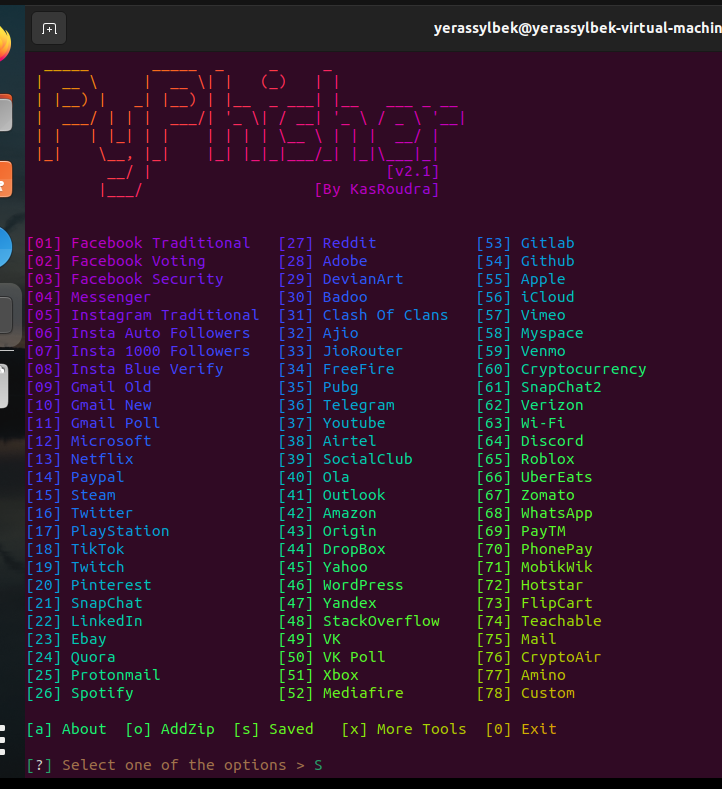
\includegraphics[scale = 0.2]{menu.png}
}
\caption{Selecting the phishing arena}
\label{fig}
\end{figure}


\subsection{share links of vulnerability}
At this point, the application provides links and we can share these links so that they are populated and we receive their data. 


\begin{figure}[htbp]
\centerline{
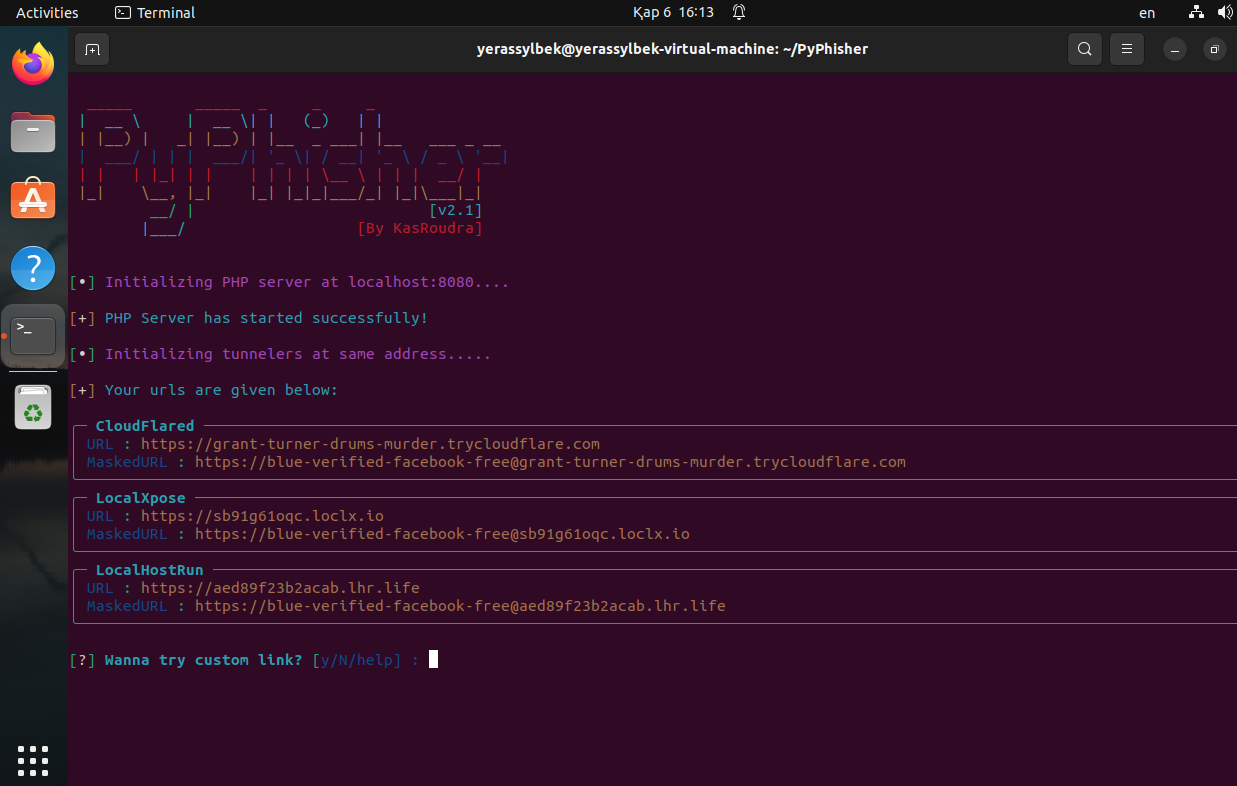
\includegraphics[scale = 0.2]{links.png}
}
\caption{Links}
\label{fig}
\end{figure}

In our case, we chose Facebook


\begin{figure}[htbp]
\centerline{
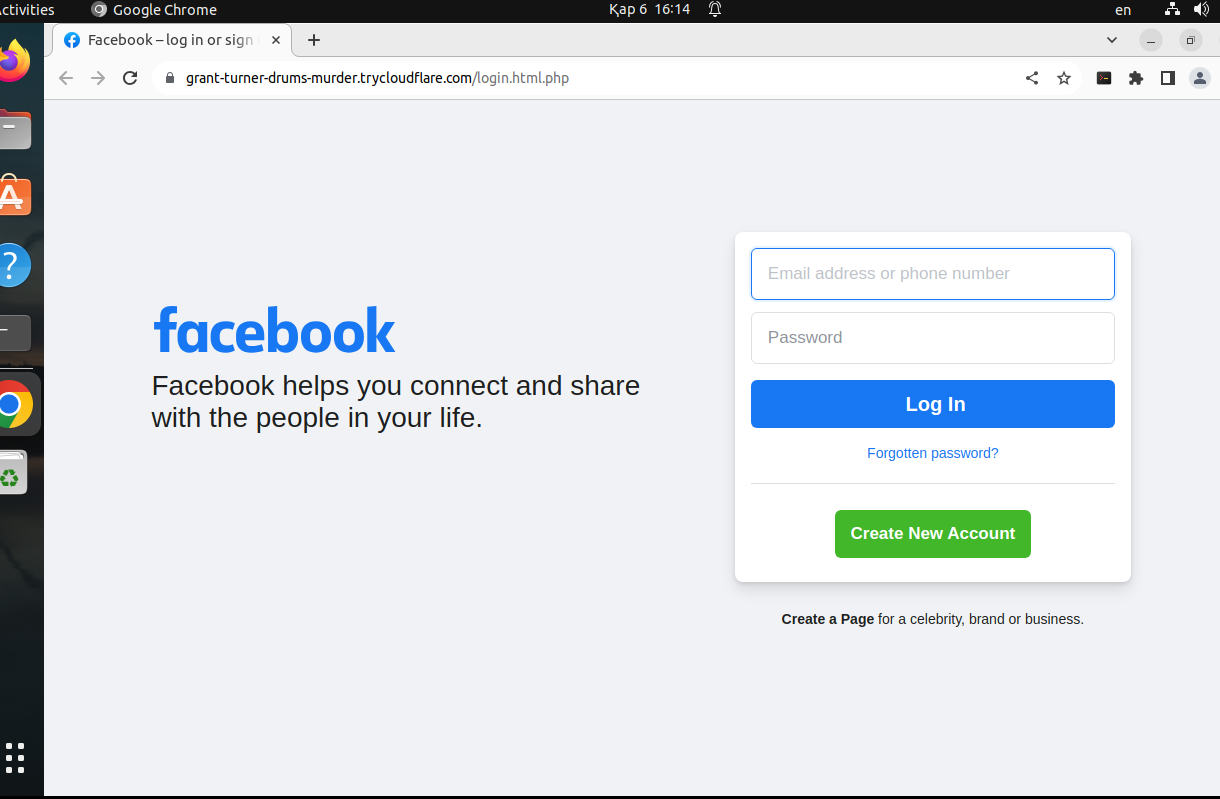
\includegraphics[scale = 0.2]{facebook.png}
}
\caption{This is what the victim sees}
\label{fig}
\end{figure}

If the victim writes something on this page, then everything he wrote will be displayed on our page. This is all scary easy!

\begin{figure}[htbp]
\centerline{
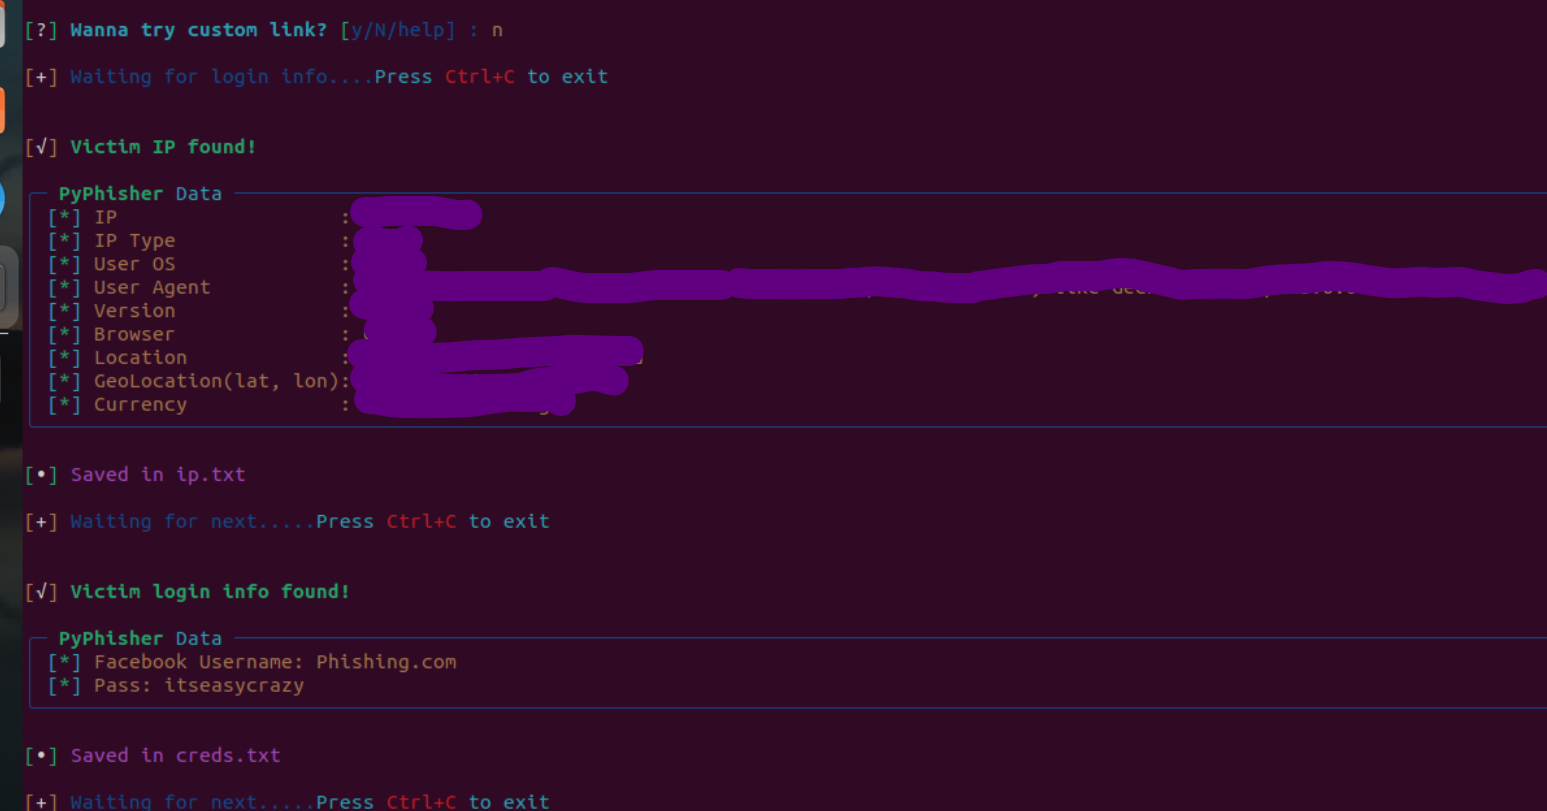
\includegraphics[scale = 0.2]{information.png}
}
\caption{This is the victim's information that we phished}
\label{fig}
\end{figure}

% llllllllllllllllllllllllllllllllllllllllllllllllllllllllllllllllllllllllllll

\section{Conclusion}

\subsection{Summary of Findings}
This comprehensive analysis has highlighted the critical importance of addressing phishing attacks in corporate environments. The key findings of this research paper are as follows:
\begin{itemize}
    \item Phishing attacks pose a substantial and evolving threat to organizations, with various attack types and tactics continually emerging.
\item Training methods, such as employee awareness training, simulated phishing exercises, and technology-based training, play a vital role in enhancing employee knowledge and vigilance against phishing threats.
\item  Campaign strategies, including email filtering, multi-factor authentication, and well-defined incident response plans, are essential components in the defense against phishing attacks.
\item  Combining effective training methods and campaign strategies can significantly improve an organization's resilience against phishing threats.
\item  Challenges and limitations, such as resource constraints, the need to adapt to new threats, and the influence of human factors, need to be carefully considered when implementing protective measures.
\end{itemize}


\subsection{Recommendations}
Based on our findings, we offer the following recommendations to help organizations strengthen their phishing protection strategies:

\begin{itemize}
    \item Prioritize employee awareness training to ensure that employees are well-informed about the risks and consequences of phishing attacks.
\item  Implement regular simulated phishing exercises to test and reinforce employee vigilance.
\item  Foster a security-conscious organizational culture that encourages employees to report suspicious activities.
\item  Utilize technology-based training tools to educate employees efficiently and keep them updated on evolving threats.
\item  Deploy robust email filtering and whitelisting solutions to reduce the influx of phishing emails.
\item  Mandate multi-factor authentication to protect against stolen credentials.
\item  Develop and regularly update incident response plans to effectively manage and mitigate phishing incidents.
\item  Explore collaborative approaches, such as sharing threat intelligence with external organizations, to enhance your security posture.
\item  Continuously monitor and improve your training methods and campaign strategies to adapt to new threats and challenges.
\item  Engage employees in the security process by encouraging their active participation and reporting of potential threats.
\end{itemize}

\subsection{Future Research Directions}
Phishing attacks and the cybersecurity landscape continue to evolve. Future research in this area should focus on the following areas:

\begin{itemize}
    \item Investigating emerging phishing tactics and techniques to stay ahead of evolving threats.
\item  Exploring innovative training methods and technologies for enhanced employee education and awareness.
\item Assessing the long-term effectiveness and sustainability of phishing protection strategies.
\item  Investigating the impact of regulatory and compliance requirements on phishing protection measures.
\item  Analyzing the economic implications of phishing attacks on organizations and the potential return on investment in prevention measures
\end{itemize}

In a constantly changing threat landscape, ongoing research and adaptation are essential for organizations to maintain effective phishing protection. This paper provides a foundation for further study and action, enabling organizations to safeguard their sensitive information and data from the persistent threat of phishing attacks.






\begin{thebibliography}{00}
\bibitem{b1} Anderson, C. (2020). Cybersecurity 101: How to Protect Your Business from Phishing Attacks. Forbes. https://www.forbes.com/sites/forbestechcouncil/2020/09/10/cybersecurity-101-how-to-protect-your-business-from-phishing-attacks/?sh=6b0bb6bf3f8c

\bibitem{b2} Barracuda. (2021). 2021 Email Security Threat Report. Barracuda Networks. https://www.barracuda.com/resources/files/whitepapers/Barracuda-Email-Security-Insights-Report-2021.pdf

\bibitem{b3} FBI. (2022). Business Email Compromise. Federal Bureau of Investigation. https://www.fbi.gov/scams-and-safety/common-scams-and-crimes/business-email-compromise

\bibitem{b4} NIST. (2020). Phishing Campaigns Targeting Unemployment Benefits in U.S. National Cybersecurity and Communications Integration Center. 

\bibitem{b5} SANS Institute. (2020). What is Spear Phishing? SANS Institute. https://www.sans.org/security-awareness-training/blog/what-spear-phishing
\bibitem{b6} Verizon. (2021). 2021 Data Breach Investigations Report. Verizon Communications. https://enterprise.verizon.com/resources/reports/dbir/
\bibitem{b7} Federal Trade Commission (FTC). (2020). How to Recognize and Avoid Phishing Scams. https://www.consumer.ftc.gov/articles/how-recognize-and-avoid-phishing-scams

\bibitem{8} Google. (2021). Protect Your Business from Phishing Scams. https://support.google.com/a/answer/9281892?hl=en

\bibitem{9} Microsoft. (2022). Multi-factor authentication for your Microsoft 365 account. Microsoft 365. https://learn.microsoft.com/en-us/mem/protect/identity/mfa-protect-your-organization

\bibitem{10} Krebs, B. (2019). The 15 Most Influential Phishing Attacks of 2019. Krebs on Security. https://krebsonsecurity.com/2020/01/the-15-most-influential-phishing-attacks-of-2019/

\end{thebibliography}

\textbf{GITHUB LINK:} 

https://github.com/keblyssareY/phishingRMT.git
\end{document}
